\section{Modeling probabilistic design}
\label{sect:prob-formulation}

To verify a deterministic design,
properties are often asserted at the primary outputs of a circuit to examine whether
there exists an assignment to the primary inputs that falsifies some of the properties.
If there exists such an assignment,
a counterexample to a property is found.

However, when it comes to probabilistic design,
the same approach is not fully adequate.
Since a probabilistic circuit could produce different output responses for the same input stimulus,
computing the probability of property violation is more meaningful than searching for a counterexample.
Hence we pose the following question:
\textit{
    Given a probabilistic circuit and a property to be verified,
    what is the average or maximum probability for the property to be violated?
}
We model a probabilistic design as a probabilistic Boolean network and
formalize \textit{probabilistic property evaluation} (PPE) to answer the question.
While the evaluation of combinational probabilistic design is of our primary interest,
the proposed framework is also extensible to sequential probabilistic design.

\subsection{Probabilistic Boolean network}
We define a probabilistic Boolean network to model circuits with logic gates that exhibit probabilistic behavior.
A \textit{probabilistic Boolean network} (PBN) is a Boolean network $G=(V,E)$ with random variables annotated to its vertices.
The probabilistic behavior of a PI $v \in V_I$ is modeled by a Bernoulli random variable
$B_v\sim\textit{Bernoulli}(p_v)$ with $p_v=\Pr[v=\top]$.
The probabilistic behavior of the output of a vertex $v \in V\setminus V_I$ is modeled with a Bernoulli random variable $B_v\sim\textit{Bernoulli}(p_v)$ with $p_v$ corresponding to the error rate of $v$.

In general,
two random variables $B_u$ and $B_v$ for $u,v \in V$ and $u \neq v$ can be dependent,
and their joint distribution has to be considered.
In this paper,
we first focus on the simplified situation where the random variables of vertices are mutually independent,
and refer to a PBN whose random variables are mutually independent as an \textit{independent PBN}.
We will show how to extend the proposed framework to a PBN with mutually dependent random variables later.

\begin{figure}[t]
    \centering
    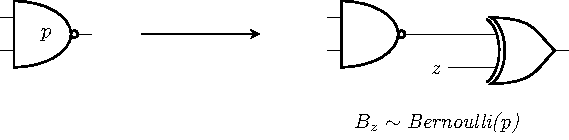
\includegraphics{fig/build/prob-distillation.pdf}
    \caption{Distillation of a \nand gate with an error rate $p$}
    \label{fig:prob-distillation}
\end{figure}

Given a PBN $G=(V,E)$,
without loss of generality,
we standardize $G$ by converting it to a \textit{standardized PBN} (SPBN) $G'=(V',E')$
with the \textit{distillation operation} depicted in~\cref{fig:prob-distillation},
using an erroneous \nand gate as an example.
For each node $v \in V\setminus V_I$ of $G$ with an error rate $p_v$,
its probabilistic behavior is distilled into an error source modeled by an auxiliary Boolean input $z$
with $B_z\sim\textit{Bernoulli}(p_v)$ for $\Pr[z=\top]=p_v$.
Moreover, an \xor gate is used to conditionally invert the output of the error-free node $v$
if and only if $z$ valuates to $\top$.
Note that an auxiliary input differs from a primary input in that
the error rate $p_z$ of an auxiliary input is fixed with respect to the characteristics of a probabilistic node
rather than determined by the environmental input behavior.
In the following, we let $V_Z$ be the set of auxiliary inputs (AIs) of an SPBN.

\subsection{Probabilistic property evaluation}
To formally reason about probabilistic design,
we formulate \textit{probabilistic property evaluation} (PPE) by capturing the degree of property violation with probability.
We distinguish between \textit{input assignment} and \textit{parameter assignment} in PPE.
An \textit{input assignment} assigns a truth value to a Boolean variable $v$ for every PI.
On the other hand,
a \textit{parameter assignment} specifies a probability $p_v$ for a PI $v$ to be \textsc{true}.
Note that the probability of an error source $z \in V_Z$ is determined by the underlying PBN and needs not be assigned.

To analyze a probabilistic design,
we define \textit{signal probability} as follows.
\begin{definition}[Signal Probability (parameterized)]
    \label{def:prob-signal-prob}
    Given an SPBN $G=(V,E)$ and a parameter assignment $\pi:V_I\mapsto[0,1]$,
    the \textit{signal probability} or \textit{satisfying probability} of a node $v \in V$
    with respect to the parameter assignment $\pi$ is $\Pr[v=\top]$ under $\pi$.
\end{definition}
It is natural to ask under what parameter assignment the signal probability of some node is maximized.
It corresponds to the following definition.
\begin{definition}[Signal Probability (maximized)]
    \label{def:prob-signal-prob-max}
    Given an SPBN $G=(V,E)$,
    the \textit{maximum signal probability} or \textit{maximum satisfying probability} of a node
    $v\in V$ is $\Pr[v=\top]$ maximized over all parameter assignments.
\end{definition}

Notice that, given a parameter assignment to the PIs of an SPBN $G=(V,E)$,
we could associate a random variable $R_v\sim\textit{Bernoulli}(p)$ with each node $v \in V$
such that $p=\Pr[v=\top]$ under $\pi$.
Those random variables can be mutually dependent (even for an SPBN derived from an independent PBN)
due to the reconvergent paths in the Boolean network.

According to~\cref{def:prob-signal-prob-max},
we have the following proposition on parameter assignments that maximize signal probability.

\begin{proposition}
    Given an SPBN $G=(V,E)$ and an arbitrary $v \in V$,
    there exists a parameter assignment $\pi$ that maximizes the signal probability of $v$
    such that $\pi(u)$ equals either probability 0 or 1 for any $u \in V_I$.
\end{proposition}
\begin{proof}
    Assume there exists an optimal parameter assignment $\pi$ not in such a form.
    That is, there exists some $u \in V_I$ such that $0<\pi(u)<1$.
    Denote the signal probabilities of $v$ under $\pi(u)=0$ and $\pi(u)=1$ by $p_0$ and $p_1$, respectively.
    Note that $\Pr[v=\top]$ under $\pi$ equals $(1-\pi(u)) \times p_0 + \pi(u) \times p_1$,
    and $\min\{p_0,p_1\}\leq\Pr[v=\top]\leq\max\{p_0,p_1\}$.
    If $p_0 \neq p_1$,
    there is a contradiction since $\Pr[v=\top]<\max\{p_0,p_1\}$,
    and $\pi$ is not an optimal assignment.
    If $p_0=p_1$, W.L.O.G., set $\pi(u)=0$.
    So the optimal assignment must be in the stated form.
\end{proof}

\begin{figure}[t]
    \centering
    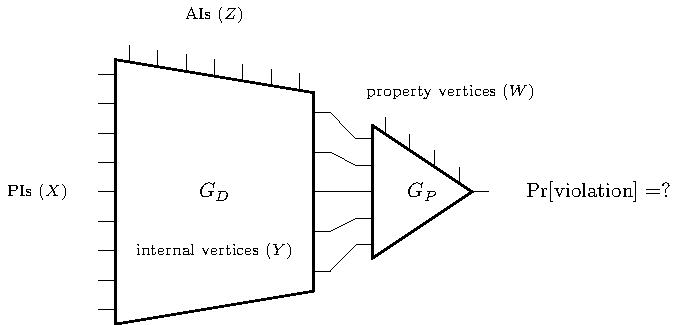
\includegraphics{fig/build/prob-spbn-miter.pdf}
    \caption{A miter SPBN for probabilistic property evaluation}
    \label{fig:prob-spbn-miter}
\end{figure}

To formulate the PPE problem,
we construct a \textit{miter SPBN} as shown in~\cref{fig:prob-spbn-miter}.
Given a \textit{design SPBN} $G_D$ modeling a probabilistic circuit and
a \textit{property SPBN} $G_P$ specifying a property under verification,
a miter SPBN $G_M$ is built by connecting relevant primary outputs of $G_D$ to the primary inputs of $G_P$.
The property SPBN is used to monitor the design SPBN.
Let $X$ be the set of PIs of $G_D$,
$Z$ be the set of AIs of $G_D$,
$W$ be a subset of PIs of $G_P$,
and $Y$ be the set of all other vertices.
Note that $G_P$ may have additional inputs $W$ to enrich the expressiveness of property.
For example, they can be used to prioritize the primary outputs of $G_D$.
Based on signal probability,
two versions of the PPE problem are defined below.

\begin{definition}[PPE (maximized)]
    Given a miter SPBN $G_M$ with the vertex sets $X,Y,Z,W$ defined as above,
    the \textit{maximum probabilistic property evaluation} (MPPE) problem asks to find the maximum satisfying probability of the output of $G_M$.
    That is,
    the signal probability of the miter output corresponds to the maximum probability of property violation under all parameter assignments.
\end{definition}

\begin{definition}[PPE (parameterized)]
    Given a miter SPBN $G_M$ with the vertex sets $X,Y,Z,W$ defined as above and a parameter assignment $\pi:X\mapsto[0,1]$,
    the \textit{probabilistic property evaluation} (PPE) problem asks to find the satisfying probability of the output of $G_M$.
    That is,
    the signal probability of the miter output corresponds to the probability of property violation under the given parameter assignment.
\end{definition}

\subsection{Extension to sequential probabilistic design}
Although the above PPE and MPPE frameworks mainly focus on combinational design,
they are extensible to analyze sequential design by \textit{circuit unrolling}~\cite{Clarke2001},
similar to the soft-error reliability analysis for sequential circuits~\cite{Miskov-Zivanov2008}.
For example,
to find the probability of property violation after $T$ clocks of execution,
the sequential circuit is \textit{unrolled} into a combinational circuit by connecting $T$ copies of the combinational block of the sequential circuit to mimic the state transitions in $T$ time frames.
For simplicity,
the occurrences of errors among different time frames are assumed to be temporally independent,
i.e., the random variables governing the probabilistic behavior of errors among different time frames are mutually independent.
After unrolling,
the proposed PPE and MPPE frameworks can be applied to the effective combinational circuit and
analyze the satisfying probability of the output at the $T^\mathrm{th}$ time frame.
The result corresponds to the probability of property violation of the sequential design after $T$ clocks of execution.